%%
%% Camera-ready submissions do not need line numbers, and
%% should have this option removed.
%%

\documentclass[11pt,lineno]{manuscript}\usepackage[]{graphicx}\usepackage[]{xcolor}
% maxwidth is the original width if it is less than linewidth
% otherwise use linewidth (to make sure the graphics do not exceed the margin)
\makeatletter
\def\maxwidth{ %
  \ifdim\Gin@nat@width>\linewidth
    \linewidth
  \else
    \Gin@nat@width
  \fi
}
\makeatother

\definecolor{fgcolor}{rgb}{0.345, 0.345, 0.345}
\newcommand{\hlnum}[1]{\textcolor[rgb]{0.686,0.059,0.569}{#1}}%
\newcommand{\hlsng}[1]{\textcolor[rgb]{0.192,0.494,0.8}{#1}}%
\newcommand{\hlcom}[1]{\textcolor[rgb]{0.678,0.584,0.686}{\textit{#1}}}%
\newcommand{\hlopt}[1]{\textcolor[rgb]{0,0,0}{#1}}%
\newcommand{\hldef}[1]{\textcolor[rgb]{0.345,0.345,0.345}{#1}}%
\newcommand{\hlkwa}[1]{\textcolor[rgb]{0.161,0.373,0.58}{\textbf{#1}}}%
\newcommand{\hlkwb}[1]{\textcolor[rgb]{0.69,0.353,0.396}{#1}}%
\newcommand{\hlkwc}[1]{\textcolor[rgb]{0.333,0.667,0.333}{#1}}%
\newcommand{\hlkwd}[1]{\textcolor[rgb]{0.737,0.353,0.396}{\textbf{#1}}}%
\let\hlipl\hlkwb

\usepackage{framed}
\makeatletter
\newenvironment{kframe}{%
 \def\at@end@of@kframe{}%
 \ifinner\ifhmode%
  \def\at@end@of@kframe{\end{minipage}}%
  \begin{minipage}{\columnwidth}%
 \fi\fi%
 \def\FrameCommand##1{\hskip\@totalleftmargin \hskip-\fboxsep
 \colorbox{shadecolor}{##1}\hskip-\fboxsep
     % There is no \\@totalrightmargin, so:
     \hskip-\linewidth \hskip-\@totalleftmargin \hskip\columnwidth}%
 \MakeFramed {\advance\hsize-\width
   \@totalleftmargin\z@ \linewidth\hsize
   \@setminipage}}%
 {\par\unskip\endMakeFramed%
 \at@end@of@kframe}
\makeatother

\definecolor{shadecolor}{rgb}{.97, .97, .97}
\definecolor{messagecolor}{rgb}{0, 0, 0}
\definecolor{warningcolor}{rgb}{1, 0, 1}
\definecolor{errorcolor}{rgb}{1, 0, 0}
\newenvironment{knitrout}{}{} % an empty environment to be redefined in TeX

\usepackage{alltt}
%\setlength{\mathindent}{0pt}
%%\usepackage{setspace}
%%\doublespacing
\usepackage{soul}
\usepackage{hyperref}
\hypersetup{
    colorlinks=true,
    linkcolor=blue,
    filecolor=blue,      
    urlcolor=blue,
    citecolor=blue,
    }


\newcommand{\beginsupplement}{%
        \setcounter{table}{0}
        \renewcommand{\thetable}{S\arabic{table}}%
        \setcounter{figure}{0}
        \renewcommand{\thefigure}{S\arabic{figure}}%
     }

\title{Template for manuscript}

\author[1]{Author One}
\author[1]{Author Two}
\author[2,3]{Author Three}
\author[1]{Author Four}
\affil[1]{Author one affiliation}
\affil[2]{Author two affiliation}
\affil[3]{Author three affiliation}

\corrauthor[1]{Author Four}{email@address}

\keywords{Keyword1; Keyword2; Keyword3}

\begin{abstract}
This is the abstract.
\end{abstract}

%%%%%%%%%%%%%%%%%%%%%%%%%%%%%%%%%%%%%%%%%%
% R specifications

%%%%%%%%%%%%%%%%%%%%%%%%%%%%%%%%%%%%%%%%%%

\IfFileExists{upquote.sty}{\usepackage{upquote}}{}
\begin{document}

\flushbottom
\maketitle
\thispagestyle{empty}

\section*{Introduction}
...

%%%%%%%%%%%%%%%%%%%%%%%%%%%%%%%%%%%%%%%%%%
\section*{Materials and Methods}
...

%%%%%%%%%%%%%%%%%%%%%%%%%%%%%%%%%%%%%%%%%%
\section*{Results}
...
 
%%%%%%%%%%%%%%%%%%%%%%%%%%%%%%%%%%%%%%%%%%
\section*{Discussion}
...

%%%%%%%%%%%%%%%%%%%%%%%%%%%%%%%%%%%%%%%%%%
\section*{Conclusions}
...

%%%%%%%%%%%%%%%%%%%%%%%%%%%%%%%%%%%%%%%%%%
\section*{Author contributions}
...

\section*{Institutional review}
...

\section*{Data availability} 
...

\section*{Funding}
...

\section*{Acknowledgments}
...

\section*{Conflicts of interest}
...

%%%%%%%%%%%%%%%%%%%%%%%%%%%%%%%%%%%%%%%%%%

\bibliography{main}

%%%%%%%%%%%%%%%%%%%%%%%%%%%%%%%%%%%%%%%%%%

\clearpage

\beginsupplement
\renewcommand\figurename{Supplementary Figure}
\renewcommand\tablename{Supplementary Table}

\section*{Appendix}

\subsection{Study design and setup} \label{subsec:design}

In 2019, 12 glacial lakes ($N =$ 12) were chosen for an experiment near Narsarsuaq,
Greenland (61.1567\textdegree{}N, -45.4254\textdegree{}E).
These glacial lakes vary in area (0.21 to 1.82 hectares) and maximum
depth (2 to 8 m), but are all clustered within a few
kilometers of each other. All lakes were fishless at the beginning of the experiment.
Six lakes were subsequently introduced with three-spined sticklebacks
(\textit{Gasterosteus aculeatus}) from nearby lakes.
Lake B1P1, B2P2, and B3P3 were introduced with \textit{Gasterosteus aculeatus} from a single
population (lake L26, 61.253333\textdegree{}N, -45.529141\textdegree{}E),
while lake B2P3, B3P1, and B3P2 were introduced with \textit{Gasterosteus aculeatus} from
two populations (lake L26, 61.253333\textdegree{}N, -45.529141\textdegree{}E
and lake ERL33, 61.118369\textdegree{}N, -45.580845\textdegree{}E).
The remaining six lakes B1P4, B2P4, B3P0, ERL85, ERL122, and ERL152 were
used as fishless control. For the purpose of this study, the origin
of the introduced \textit{Gasterosteus aculeatus} is of minor importance,
as they all originate from the same area (Supplementary Table~\ref{tab:lakes}).

In 2021, 2022, and 2023, all 12 lakes were monitored over several days.
For that purpose, EXO2 multiparameter sondes were installed
(YSI, Yellow Springs, OH, USA), tracking ecosystem parameters with high
frequency (2-minute intervals in 2021 and 2022, 5-minute intervals in
2023 with the exception of ERL122, which was monitored in 15-minute intervals).
For the purpose of this study, only dissolved oxygen (hereafter DO) and temperature measurements
yielded from these sondes are relevant. The sensors were situated at a water depth
of approximately 1-1.5 m in each lake. All optical sensors were
wiped clean before every measurement with a built-in wiper.
The monitoring period was 16 September-24 September in 2021, 22 June-3 July in 2022,
and 22 June-17 July in 2023.

% latex table generated in R 4.4.1 by xtable 1.8-4 package
% Tue Dec 10 16:08:53 2024
\begin{table}[ht]
\centering
\caption{Lakes included in the experiment, along with treatment
                and general characteristics.} 
\label{tab:lakes}
\begin{tabular}{lllllll}
  \toprule
Lake & Treatment & Latitude (°N) & Longitude (°E) & Altitude (m) & Area (hectare) & Maximum Depth (m) \\ 
  \midrule
B1P1 & Fish & 61.15338 & -45.57081 & 272 & 0.21 & 4.00 \\ 
  B2P2 & Fish & 61.12299 & -45.55988 & 255 & 0.50 & 3.00 \\ 
  B3P3 & Fish & 61.13385 & -45.57556 & 258 & 0.30 & 5.00 \\ 
  B2P3 & Fish & 61.12275 & -45.55696 & 261 & 0.41 & 4.25 \\ 
  B3P1 & Fish & 61.13130 & -45.51195 & 180 & 0.40 & 2.00 \\ 
  B3P2 & Fish & 61.12788 & -45.51031 & 201 & 0.53 & 4.50 \\ 
  B1P4 & No Fish & 61.16552 & -45.56801 & 304 & 0.44 & 2.20 \\ 
  B2P4 & No Fish & 61.12192 & -45.55497 & 261 & 0.51 & 7.00 \\ 
  B3P0 & No Fish & 61.13210 & -45.51416 & 177 & 0.81 & 4.00 \\ 
  ERL85 & No Fish & 61.14171 & -45.59328 & 120 & 1.82 & 8.00 \\ 
  ERL122 & No Fish & 61.14182 & -45.53623 & 111 & 1.10 & 5.00 \\ 
  ERL152 & No Fish & 61.14646 & -45.59235 & 156 & 0.73 & 4.50 \\ 
   \bottomrule
\end{tabular}
\end{table}


\subsection{Data sources} \label{subsec:source}

DO ($mg\,L^{-1}$) and water temperature (\textdegree{}$C$) measurements
were yielded from EXO2 multiparameter
sondes, as described in section~\nameref{subsec:design}. For the purpose
of estimating ecosystem metabolism, wind and irradiation data were yielded
from the Programme for Monitoring of the Greenland Ice Sheet (PROMICE), providing automatic
weather station data \citep{Fausto:2021}.
The dataset named \texttt{QAS\_L\_hour.csv} originating from the QAS\_L automated weather station
near Narsarsuaq was downloaded from a
\href{https://dataverse.geus.dk/citation?persistentId=doi:10.22008/FK2/IW73UU}{public database}
provided by PROMICE \citep{metadata}.
Wind data was provided as average wind speed in hourly intervals ($m\,s^{-1}$), while
irradiation was provided as downwelling shortwave irradiation additionally
corrected for the tilt of the sensor ($W\,m^{-2}$).

\subsection{Data pipeline} \label{subsec:pipeline}

The data preparation and analysis for estimating lake metabolism was done separately for each monitoring
period (16 September-24 September 2021, 22 June-3 July 2022, and 22 June-17 July 2023).

First, the raw sonde data from each lake were imported and merged into
one dataset for a given monitoring period. The variables required for lake metabolism
estimation were water temperature and
DO. Next, an outlier analysis was performed by removing
values higher than three times the median absolute deviation of all values in a
sliding window of one day window size \citep{Luerig:2021}.
After outlier removal, the time series of water temperature and DO
were plotted and subsequently investigated for larger data gaps due to potential lack of sensor
measurements over certain periods.

To ensure overlapping estimation of lake metabolism, the data was subsequently
cut to achieve equal starting and ending time points for all lakes during a given
monitoring period. Due to large data gaps during the period of 2022, we chose
to keep as much complete days as possible in order to estimate the maximum
amount of days, rather than selecting the longest common monitoring period
for all lakes.

After cutting the sonde data, they were subsequently merged with the weather data.
Since the weather data were collected in hourly intervals, they were inflated to match
the measurement intervals of the sonde data (see section \nameref{subsec:design}).

After merging sonde and weather data, potential missing values due to outlier removal
were imputed by a weighted moving average, where the weights of observations around the
central value to be imputed decrease exponentially \citep{Moritz:2017}.
For larger data gaps spanning over several hours (due to sonde malfunction rather
than outlier removal), we chose
to not estimate lake metabolism for the affected days.\smallskip

All data preparation and analysis was done with the \texttt{R} programming language \citep{R}.
To estimate lake metabolism, the package \texttt{LakeMetabolizer} was used \citep{Winslow:2016}.
Specifically, a Bayesian framework to estimate whole lake metabolism from free-water
DO by using the function \texttt{metab.bayesian} was chosen for
this analysis \citep{Holtgrieve:2010}.
In order to be able to fit the model, a minimum of 6 variables are needed as input:

\begin{enumerate}
\item doobs: DO concentration measurements ($mg\,L^{-1}$)
\item do.sat: Equilibrium DO concentration for specific temperature ($mg\,L^{-1}$, hereafter do.sat)
\item k.gas: Gas and temperature specific gas transfer coefficient ($m^{-1}$, hereafter k.gas)
\item par: Photosynthetically active radiation ($\mu{}mol\,m^{-2}\,s^{-1}$, hereafter par)
\item z.mix: Actively mixed layer depth ($m$, hereafter z.mix)
\item wtr: Water temperature (\textdegree{}$C$)
\end{enumerate}

Some of the variables listed above have to be derived from other time series data prior
to estimating lake metabolism,
namely do.sat, k.gas, par, and z.mix.
do.sat was derived by using the function \texttt{o2.at.sat}, which calculates
the equilibrium DO concentration in water at supplied conditions.
To estimate k.gas, a gas transfer coefficient model must be fit.
The \texttt{LakeMetabolizer} package offers different methods, and we chose
an empirical wind-based gas exchange model, introduced by Vachon and
Prairie in 2013 \citep{Vachon:2013}. This model not only takes wind into
consideration, but also lake area. Notably, wind speed has to be normalized
to 10 $m$ sensor height before fitting any gas exchange model, which is achieved
with the function \texttt{wind.scale}.
All models of gas exchange 
return a k\textsubscript{600} value, a gas exchange normalized to a Schmidt 
number (Sc) of 600, or O\textsubscript{2} at 17.5 \textdegree{}$C$.
After estimating k\textsubscript{600}, it must be transformed to k.gas by using the
function \texttt{k600.2.kGAS} provided by the \texttt{LakeMetabolizer}
package. par was derived from shortwave irradiation,
which we had available (see section \nameref{subsec:source}).
To achieve this transformation, we used the function \texttt{sw.to.par},
which uses the simple empirical transformation $par = 2.114 \times sw$ \citep{Britton:1976}.
To estimate z.mix, one normally needs a time series profile of water temperature
or water density. Since we did not have such data available, we decided to
simulate actively mixed layer depth by drawing from a uniform distribution
with limits 0 and maximum depth of the lake. The reasoning behind this simulation
is that, although the simulated time series of z.mix likely differing substantially
from the actual, a possible treatment effect of fish versus no fish should still be
consistent, given the simulation is performed equally in all lakes.\smallskip

After performing the data preparation and the derivation for certain model
inputs, the Bayesian lake metabolism model was fitted for each lake and
monitoring period. The Bayesian model is special, as it considers 2 types
of errors: Differences between the true data generating process and the process
defined in the model (process error) and errors resulting from inaccuracies
of DO measurements (observation error). Reflecting this philosophy, the
Bayesian model distinguishes between 3 categories of DO values: $y$ represents
the DO measurements, $\alpha$ the true but unknown DO values, and
$\alpha^{\ast}$ the model's estimates of the true value.
The observed DO measurements $y$ are modeled as random deviations from the true
value $\alpha$:

\begin{equation}
y_{t} \sim N(\alpha_{t}, \tau_{v}),
\label{eq:doobs}
\end{equation}

where $\tau_{v}$ is the precision of the observation error (precision is
the reciprocal of variance).
Note, that the Bayesian model fits parameter values by making a comparison
between observed and theoretical values of DO.
This comparison is made in equation \ref{eq:dotrue}, where we define the true value of 
DO at time $t$, $\alpha_{t}$, as being normally distributed with mean 
$\alpha^{\ast}_{t}$ and process precision $\tau_{w}$:

\begin{equation}
\alpha_{t} \sim N(\alpha^{\ast}_{t}, \tau_{w}),
\label{eq:dotrue}
\end{equation}

where $\tau_{w}$ is the precision of the process error.
The important distinction of process and observation error is that
process error affects the state of the system at time
$t + k (k=0, 1, ..., T-t)$, because the state evolves dynamically, whereas
observation error only affects the state of the system at time $t$.

Both $\tau_{v}$ and $\tau_{w}$ are given minimally informative priors
following a gamma distribution with shape and rate parameters of 0.001.

The Bayesian model can be described by the following equations:

\begin{gather}
\alpha^{\ast}_{t} =
\begin{cases}
\alpha_{t-1} + \alpha_{t}, & \text{if } k_{t} = 0, \\
\frac{\alpha_{t}}{k_{t-1}} + \frac{-\exp{(-k_{t-1})}\alpha_{t}}{k_{t-1}} +
\exp{(-k_{t-1})}\alpha_{t-1}, & \text{otherwise},
\end{cases} \label{eq:sys1} \\
\alpha_{t} = \mathbf{X}_{t-1}\bm{\beta} + k_{t-1}O_{s,t-1}, \label{eq:sys2} \\
k_{t} = \frac{K^{\ast}_{t}\Delta t}{z_{t}}. \label{eq:sys3}
\end{gather}

In this equation structure, $k_{t}$ is the coefficient of gas exchange;
$\mathbf{X}$ is an $n \times 2$ matrix of predictor variables with $I$
(irradiation in arbitrary light units) in the first column and $\ln{T}$ (\textdegree{}$C$) in the second
column; $\bm{\beta}$ is a $2 \times 1$ vector of parameters to be estimated
($\iota$, $\rho$). $\iota$ represents the parameter for Gross Primary Production
(hereafter GPP), implying a linear relationship between GPP and irradiation, and $\rho$ represents
the parameter for Respiration (hereafter R), implying a log-linear relationship
between R and temperature; $O_{s}$ is the equilibrium DO concentration at
supplied conditions; $K^{\ast}_{t}$ is a stochastic node,
with $K^{\ast}_{t} \sim N(K_{t}, \sigma_{k})$, where $K_{t}$ is the gas exchange
coefficient, and $\sigma_{k}$ the precision thereof; the default precision
is $1/(0.1 \times K_{t})$; finally, $z_{t}$ is the mixed layer depth.

From equation~\ref{eq:sys1}, we can see that if $k_{t} = 0$ (i.e., no gas exchange
with the atmosphere), the oxygen levels in the water are modeled to be additive for each
time step. Furthermore, we can see that the gas exchange coefficient is dependent
on mixed layer depth (equation~\ref{eq:sys3}).

While the estimate of gas exchange coefficient serves as prior information for $K$,
priors for the fitted GPP and R parameters ($\iota$ and $\rho$) can also
be defined. The default priors for $\iota$ and $\rho$ are normal distributions
with mean 0 and variance $1 \times 10^{5}$
($\iota_{t} \sim N(0,10^{5})$, $\rho_{t} \sim N(0,10^{5})$) and were used in our case.

To estimate metabolism, the median of the posterior distribution of the parameters
is used as a scalar estimate. Daily GPP and R estimates represent an integrated
estimate of these scalars over a 24-hour window. Uncertainty of GPP and R
estimates is expressed as the posterior standard deviation of the respective
parameters ($\iota$ and $\rho$), multiplied by the square root of the corresponding
covariate ($I$ and $\ln{T}$). NEP is the sum of GPP and R, and the standard deviation
of NEP is the sum of the standard deviations for GPP and R.

In total, 5 parameters are fit in this Bayesian model, namely $\iota$, $\rho$,
$K$, $\tau_{v}$, and $\tau_{w}$. For all parameters except $K$, (default) minimally
informative priors were used. Regarding $K$, as described above, its estimate
(from the separate gas transfer coefficient model) serves as a prior.

Estimates of the posterior distribution of the parameters were sampled using
Gibbs sampling implemented in Just Another Gibbs Sampler
(\href{https://sourceforge.net/projects/mcmc-jags/files/}{JAGS}). Prior to running
the Bayesian model, it must be installed.

\subsection{Sensitivity analysis for mixed layer depth} \label{subsec:sens}

As mentioned in section~\nameref{subsec:pipeline}, we did not have the necessary
data to estimate mixed layer depth. An initial approach to deal with that problem
was to investigate the effect of different mixed layer depths on the daily metabolism
estimates. For that purpose, we selected a few lakes for different monitoring
periods (2021, 2022, 2023) and assessed the impact of various, constant
mixed layer depths over time on the metabolism results.

\begin{kframe}


{\ttfamily\noindent\itshape\color{messagecolor}{\#\# Lade nötiges Paket: grid}}\end{kframe}datetime  dsr_cor      wsp     Pond   do.obs      wtr 
       0        0        0        0      154        0 
[1] 0


{\centering 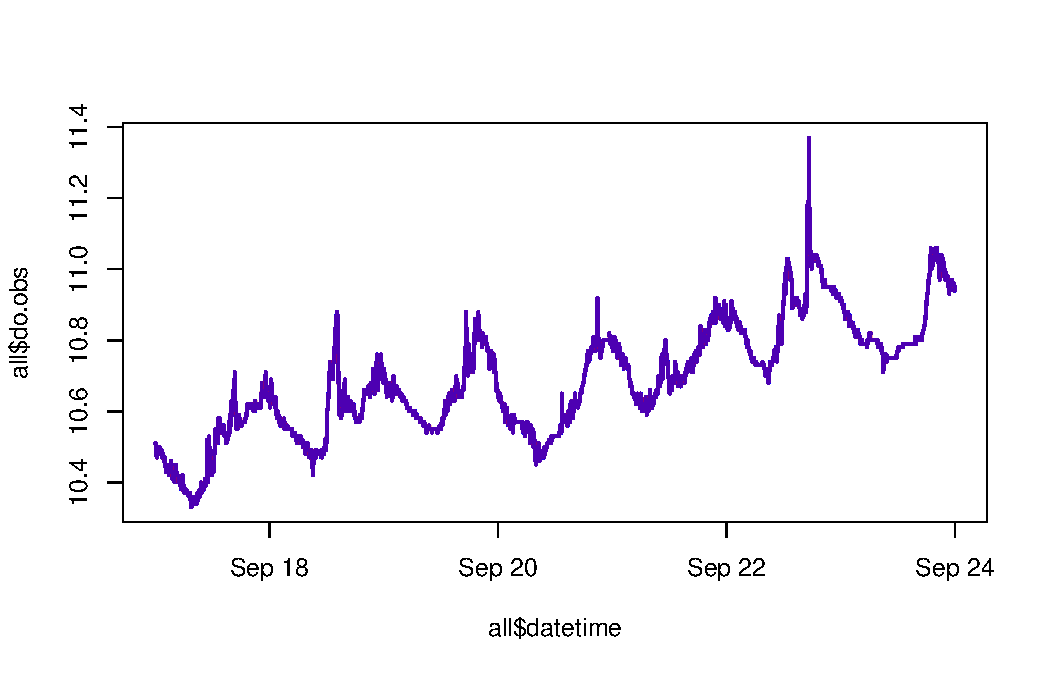
\includegraphics[width=\maxwidth]{plots/psensanal-1} 

}


[1] 0
[1] "Points removed due to incomplete day or duplicated time step: 0"
[1] "NA's added to fill in time series: 0"
[1] "using allK model"
\begin{kframe}

{\ttfamily\noindent\itshape\color{messagecolor}{\#\# module glm loaded}}\end{kframe}Compiling model graph
   Resolving undeclared variables
   Allocating nodes
Graph information:
   Observed stochastic nodes: 719
   Unobserved stochastic nodes: 1442
   Total graph size: 16998

Initializing model

[1] "using allK model"
Compiling model graph
   Resolving undeclared variables
   Allocating nodes
Graph information:
   Observed stochastic nodes: 719
   Unobserved stochastic nodes: 1442
   Total graph size: 16988

Initializing model

[1] "using allK model"
Compiling model graph
   Resolving undeclared variables
   Allocating nodes
Graph information:
   Observed stochastic nodes: 719
   Unobserved stochastic nodes: 1442
   Total graph size: 16925

Initializing model

[1] "using allK model"
Compiling model graph
   Resolving undeclared variables
   Allocating nodes
Graph information:
   Observed stochastic nodes: 719
   Unobserved stochastic nodes: 1442
   Total graph size: 17003

Initializing model

[1] "using allK model"
Compiling model graph
   Resolving undeclared variables
   Allocating nodes
Graph information:
   Observed stochastic nodes: 719
   Unobserved stochastic nodes: 1442
   Total graph size: 17076

Initializing model

[1] "using allK model"
Compiling model graph
   Resolving undeclared variables
   Allocating nodes
Graph information:
   Observed stochastic nodes: 719
   Unobserved stochastic nodes: 1442
   Total graph size: 16921

Initializing model

[1] "using allK model"
Compiling model graph
   Resolving undeclared variables
   Allocating nodes
Graph information:
   Observed stochastic nodes: 719
   Unobserved stochastic nodes: 1442
   Total graph size: 16947

Initializing model

[1] "Points removed due to incomplete day or duplicated time step: 0"
[1] "NA's added to fill in time series: 0"
[1] "using allK model"
Compiling model graph
   Resolving undeclared variables
   Allocating nodes
Graph information:
   Observed stochastic nodes: 719
   Unobserved stochastic nodes: 1442
   Total graph size: 16998

Initializing model

[1] "using allK model"
Compiling model graph
   Resolving undeclared variables
   Allocating nodes
Graph information:
   Observed stochastic nodes: 719
   Unobserved stochastic nodes: 1442
   Total graph size: 16988

Initializing model

[1] "using allK model"
Compiling model graph
   Resolving undeclared variables
   Allocating nodes
Graph information:
   Observed stochastic nodes: 719
   Unobserved stochastic nodes: 1442
   Total graph size: 16925

Initializing model

[1] "using allK model"
Compiling model graph
   Resolving undeclared variables
   Allocating nodes
Graph information:
   Observed stochastic nodes: 719
   Unobserved stochastic nodes: 1442
   Total graph size: 17003

Initializing model

[1] "using allK model"
Compiling model graph
   Resolving undeclared variables
   Allocating nodes
Graph information:
   Observed stochastic nodes: 719
   Unobserved stochastic nodes: 1442
   Total graph size: 17076

Initializing model

[1] "using allK model"
Compiling model graph
   Resolving undeclared variables
   Allocating nodes
Graph information:
   Observed stochastic nodes: 719
   Unobserved stochastic nodes: 1442
   Total graph size: 16921

Initializing model

[1] "using allK model"
Compiling model graph
   Resolving undeclared variables
   Allocating nodes
Graph information:
   Observed stochastic nodes: 719
   Unobserved stochastic nodes: 1442
   Total graph size: 16947

Initializing model

[1] "Points removed due to incomplete day or duplicated time step: 0"
[1] "NA's added to fill in time series: 0"
[1] "using allK model"
Compiling model graph
   Resolving undeclared variables
   Allocating nodes
Graph information:
   Observed stochastic nodes: 719
   Unobserved stochastic nodes: 1442
   Total graph size: 16998

Initializing model

[1] "using allK model"
Compiling model graph
   Resolving undeclared variables
   Allocating nodes
Graph information:
   Observed stochastic nodes: 719
   Unobserved stochastic nodes: 1442
   Total graph size: 16988

Initializing model

[1] "using allK model"
Compiling model graph
   Resolving undeclared variables
   Allocating nodes
Graph information:
   Observed stochastic nodes: 719
   Unobserved stochastic nodes: 1442
   Total graph size: 16925

Initializing model

[1] "using allK model"
Compiling model graph
   Resolving undeclared variables
   Allocating nodes
Graph information:
   Observed stochastic nodes: 719
   Unobserved stochastic nodes: 1442
   Total graph size: 17003

Initializing model

[1] "using allK model"
Compiling model graph
   Resolving undeclared variables
   Allocating nodes
Graph information:
   Observed stochastic nodes: 719
   Unobserved stochastic nodes: 1442
   Total graph size: 17076

Initializing model

[1] "using allK model"
Compiling model graph
   Resolving undeclared variables
   Allocating nodes
Graph information:
   Observed stochastic nodes: 719
   Unobserved stochastic nodes: 1442
   Total graph size: 16921

Initializing model

[1] "using allK model"
Compiling model graph
   Resolving undeclared variables
   Allocating nodes
Graph information:
   Observed stochastic nodes: 719
   Unobserved stochastic nodes: 1442
   Total graph size: 16947

Initializing model

[1] "Points removed due to incomplete day or duplicated time step: 0"
[1] "NA's added to fill in time series: 0"
[1] "using allK model"
Compiling model graph
   Resolving undeclared variables
   Allocating nodes
Graph information:
   Observed stochastic nodes: 719
   Unobserved stochastic nodes: 1442
   Total graph size: 16998

Initializing model

[1] "using allK model"
Compiling model graph
   Resolving undeclared variables
   Allocating nodes
Graph information:
   Observed stochastic nodes: 719
   Unobserved stochastic nodes: 1442
   Total graph size: 16988

Initializing model

[1] "using allK model"
Compiling model graph
   Resolving undeclared variables
   Allocating nodes
Graph information:
   Observed stochastic nodes: 719
   Unobserved stochastic nodes: 1442
   Total graph size: 16925

Initializing model

[1] "using allK model"
Compiling model graph
   Resolving undeclared variables
   Allocating nodes
Graph information:
   Observed stochastic nodes: 719
   Unobserved stochastic nodes: 1442
   Total graph size: 17003

Initializing model

[1] "using allK model"
Compiling model graph
   Resolving undeclared variables
   Allocating nodes
Graph information:
   Observed stochastic nodes: 719
   Unobserved stochastic nodes: 1442
   Total graph size: 17076

Initializing model

[1] "using allK model"
Compiling model graph
   Resolving undeclared variables
   Allocating nodes
Graph information:
   Observed stochastic nodes: 719
   Unobserved stochastic nodes: 1442
   Total graph size: 16921

Initializing model

[1] "using allK model"
Compiling model graph
   Resolving undeclared variables
   Allocating nodes
Graph information:
   Observed stochastic nodes: 719
   Unobserved stochastic nodes: 1442
   Total graph size: 16947

Initializing model

[1] "Points removed due to incomplete day or duplicated time step: 0"
[1] "NA's added to fill in time series: 0"
[1] "using allK model"
Compiling model graph
   Resolving undeclared variables
   Allocating nodes
Graph information:
   Observed stochastic nodes: 719
   Unobserved stochastic nodes: 1442
   Total graph size: 16998

Initializing model

[1] "using allK model"
Compiling model graph
   Resolving undeclared variables
   Allocating nodes
Graph information:
   Observed stochastic nodes: 719
   Unobserved stochastic nodes: 1442
   Total graph size: 16988

Initializing model

[1] "using allK model"
Compiling model graph
   Resolving undeclared variables
   Allocating nodes
Graph information:
   Observed stochastic nodes: 719
   Unobserved stochastic nodes: 1442
   Total graph size: 16925

Initializing model

[1] "using allK model"
Compiling model graph
   Resolving undeclared variables
   Allocating nodes
Graph information:
   Observed stochastic nodes: 719
   Unobserved stochastic nodes: 1442
   Total graph size: 17003

Initializing model

[1] "using allK model"
Compiling model graph
   Resolving undeclared variables
   Allocating nodes
Graph information:
   Observed stochastic nodes: 719
   Unobserved stochastic nodes: 1442
   Total graph size: 17076

Initializing model

[1] "using allK model"
Compiling model graph
   Resolving undeclared variables
   Allocating nodes
Graph information:
   Observed stochastic nodes: 719
   Unobserved stochastic nodes: 1442
   Total graph size: 16921

Initializing model

[1] "using allK model"
Compiling model graph
   Resolving undeclared variables
   Allocating nodes
Graph information:
   Observed stochastic nodes: 719
   Unobserved stochastic nodes: 1442
   Total graph size: 16947

Initializing model

[1] "Points removed due to incomplete day or duplicated time step: 0"
[1] "NA's added to fill in time series: 0"
[1] "using allK model"
Compiling model graph
   Resolving undeclared variables
   Allocating nodes
Graph information:
   Observed stochastic nodes: 719
   Unobserved stochastic nodes: 1442
   Total graph size: 16998

Initializing model

[1] "using allK model"
Compiling model graph
   Resolving undeclared variables
   Allocating nodes
Graph information:
   Observed stochastic nodes: 719
   Unobserved stochastic nodes: 1442
   Total graph size: 16988

Initializing model

[1] "using allK model"
Compiling model graph
   Resolving undeclared variables
   Allocating nodes
Graph information:
   Observed stochastic nodes: 719
   Unobserved stochastic nodes: 1442
   Total graph size: 16925

Initializing model

[1] "using allK model"
Compiling model graph
   Resolving undeclared variables
   Allocating nodes
Graph information:
   Observed stochastic nodes: 719
   Unobserved stochastic nodes: 1442
   Total graph size: 17003

Initializing model

[1] "using allK model"
Compiling model graph
   Resolving undeclared variables
   Allocating nodes
Graph information:
   Observed stochastic nodes: 719
   Unobserved stochastic nodes: 1442
   Total graph size: 17076

Initializing model

[1] "using allK model"
Compiling model graph
   Resolving undeclared variables
   Allocating nodes
Graph information:
   Observed stochastic nodes: 719
   Unobserved stochastic nodes: 1442
   Total graph size: 16921

Initializing model

[1] "using allK model"
Compiling model graph
   Resolving undeclared variables
   Allocating nodes
Graph information:
   Observed stochastic nodes: 719
   Unobserved stochastic nodes: 1442
   Total graph size: 16947

Initializing model

[1] "Points removed due to incomplete day or duplicated time step: 0"
[1] "NA's added to fill in time series: 0"
[1] "using allK model"
Compiling model graph
   Resolving undeclared variables
   Allocating nodes
Graph information:
   Observed stochastic nodes: 719
   Unobserved stochastic nodes: 1442
   Total graph size: 16998

Initializing model

[1] "using allK model"
Compiling model graph
   Resolving undeclared variables
   Allocating nodes
Graph information:
   Observed stochastic nodes: 719
   Unobserved stochastic nodes: 1442
   Total graph size: 16988

Initializing model

[1] "using allK model"
Compiling model graph
   Resolving undeclared variables
   Allocating nodes
Graph information:
   Observed stochastic nodes: 719
   Unobserved stochastic nodes: 1442
   Total graph size: 16925

Initializing model

[1] "using allK model"
Compiling model graph
   Resolving undeclared variables
   Allocating nodes
Graph information:
   Observed stochastic nodes: 719
   Unobserved stochastic nodes: 1442
   Total graph size: 17003

Initializing model

[1] "using allK model"
Compiling model graph
   Resolving undeclared variables
   Allocating nodes
Graph information:
   Observed stochastic nodes: 719
   Unobserved stochastic nodes: 1442
   Total graph size: 17076

Initializing model

[1] "using allK model"
Compiling model graph
   Resolving undeclared variables
   Allocating nodes
Graph information:
   Observed stochastic nodes: 719
   Unobserved stochastic nodes: 1442
   Total graph size: 16921

Initializing model

[1] "using allK model"
Compiling model graph
   Resolving undeclared variables
   Allocating nodes
Graph information:
   Observed stochastic nodes: 719
   Unobserved stochastic nodes: 1442
   Total graph size: 16947

Initializing model

[1] "Points removed due to incomplete day or duplicated time step: 0"
[1] "NA's added to fill in time series: 0"
[1] "using allK model"
Compiling model graph
   Resolving undeclared variables
   Allocating nodes
Graph information:
   Observed stochastic nodes: 719
   Unobserved stochastic nodes: 1442
   Total graph size: 16998

Initializing model

[1] "using allK model"
Compiling model graph
   Resolving undeclared variables
   Allocating nodes
Graph information:
   Observed stochastic nodes: 719
   Unobserved stochastic nodes: 1442
   Total graph size: 16988

Initializing model

[1] "using allK model"
Compiling model graph
   Resolving undeclared variables
   Allocating nodes
Graph information:
   Observed stochastic nodes: 719
   Unobserved stochastic nodes: 1442
   Total graph size: 16925

Initializing model

[1] "using allK model"
Compiling model graph
   Resolving undeclared variables
   Allocating nodes
Graph information:
   Observed stochastic nodes: 719
   Unobserved stochastic nodes: 1442
   Total graph size: 17003

Initializing model

[1] "using allK model"
Compiling model graph
   Resolving undeclared variables
   Allocating nodes
Graph information:
   Observed stochastic nodes: 719
   Unobserved stochastic nodes: 1442
   Total graph size: 17076

Initializing model

[1] "using allK model"
Compiling model graph
   Resolving undeclared variables
   Allocating nodes
Graph information:
   Observed stochastic nodes: 719
   Unobserved stochastic nodes: 1442
   Total graph size: 16921

Initializing model

[1] "using allK model"
Compiling model graph
   Resolving undeclared variables
   Allocating nodes
Graph information:
   Observed stochastic nodes: 719
   Unobserved stochastic nodes: 1442
   Total graph size: 16947

Initializing model

$y
expression(paste("R (", O[2], " in mg L", NULL^-1, " day", NULL^-1, 
    ")"))

attr(,"class")
[1] "labels"
$y
expression(paste("NEP (", O[2], " in mg L", NULL^-1, " day", 
    NULL^-1, ")"))

attr(,"class")
[1] "labels"
\begin{kframe}

{\ttfamily\noindent\color{warningcolor}{\#\# Warning in grid.Call(C\_textBounds, as.graphicsAnnot(x\$label), x\$x, x\$y, : font metrics unknown for character 0x0a in encoding cp1252}}

{\ttfamily\noindent\color{warningcolor}{\#\# Warning in grid.Call(C\_textBounds, as.graphicsAnnot(x\$label), x\$x, x\$y, : font metrics unknown for character 0x0a in encoding cp1252}}

{\ttfamily\noindent\color{warningcolor}{\#\# Warning in grid.Call.graphics(C\_text, as.graphicsAnnot(x\$label), x\$x, x\$y, : font metrics unknown for character 0x0a in encoding cp1252}}

{\ttfamily\noindent\color{warningcolor}{\#\# Warning in grid.Call.graphics(C\_text, as.graphicsAnnot(x\$label), x\$x, x\$y, : font metrics unknown for character 0x0a in encoding cp1252}}

{\ttfamily\noindent\color{warningcolor}{\#\# Warning in grid.Call(C\_textBounds, as.graphicsAnnot(x\$label), x\$x, x\$y, : font metrics unknown for character 0x0a in encoding cp1252}}

{\ttfamily\noindent\color{warningcolor}{\#\# Warning in grid.Call(C\_textBounds, as.graphicsAnnot(x\$label), x\$x, x\$y, : font metrics unknown for character 0x0a in encoding cp1252}}

{\ttfamily\noindent\color{warningcolor}{\#\# Warning in grid.Call.graphics(C\_text, as.graphicsAnnot(x\$label), x\$x, x\$y, : font metrics unknown for character 0x0a in encoding cp1252}}

{\ttfamily\noindent\color{warningcolor}{\#\# Warning in grid.Call.graphics(C\_text, as.graphicsAnnot(x\$label), x\$x, x\$y, : font metrics unknown for character 0x0a in encoding cp1252}}\end{kframe}

{\centering 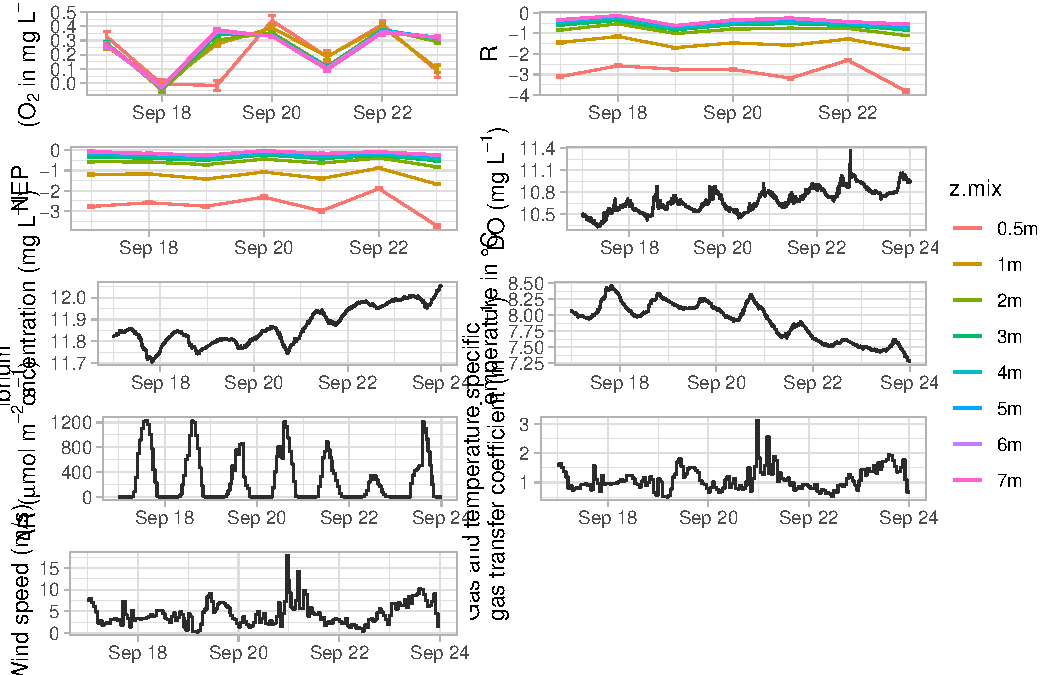
\includegraphics[width=\maxwidth]{plots/psensanal-2} 

}





















\end{document}

